% Chapter Template

\chapter{Desarrollo}

\label{Chapter4} % Change X to a consecutive number; for referencing this chapter elsewhere, use \ref{ChapterX}

Una vez presentado el contexto, los objetivos, así como las herramientas empleadas y los fundamentos teóricos, en este capítulo se detallará la solución software final desarrollada. Primero se presenta el diseño global utilizado y después se analizará en detalle el componente en cuestión realizado con una visión profunda del desarrollo por bloques y su funcionamiento.


%-----------------------------------
%	SECTION Diseño
%-----------------------------------
\section{Diseño}

El trabajo se basa principalmente en dos componentes; un componente de JDeRobot (\textbf{OpenniServer}) que funciona como driver del sensor y proporciona las imágenes obtenidas por éste y el componente realizado (\textbf{RealRTEstimator}) que se encargará, una vez recogidas las imágenes, de toda la lógica restante.

El objetivo del componente, como ya se ha comentado, consiste en analizar en tiempo real la posición y movimiento del sensor, por lo que el componente deberá dar una estimación en todo momento.

En la Figura~\ref{fig:diagram1} se puede apreciar el diagrama global de funcionamiento del componente desarrollado y su conexión con otros componentes para los diferentes datos de entrada.

\begin{figure}[th]
\centering
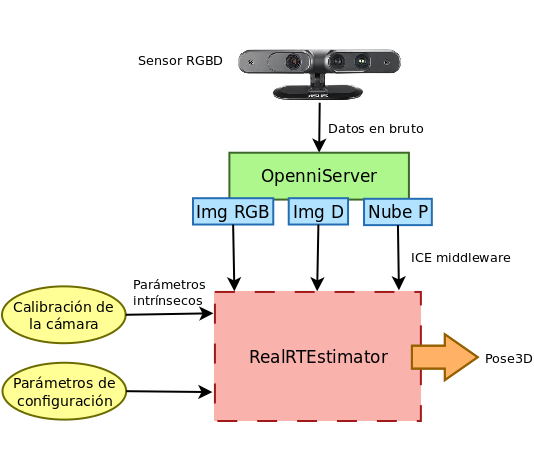
\includegraphics[scale=0.4]{Figures/diagram1.png}
\decoRule
\caption[Diagram1]{Esquema global de funcionamiento.}
\label{fig:diagram1}
\end{figure}

OpenniServer se encarga de preparar y enviar las imágenes del sensor. El componente recoge las imágenes a través de ICE y éste es el encargado de procesarlas. También recibe los datos de los parámetros intrínsecos de la cámara así como algunos parámetros de configuración, como pueden ser la activación/desactivación de la interfaz de usuario o algunos parámetros configurables de algunos de los algoritmos internos. A su salida entrega una matriz RT que describe la posición y orientación absolutas en ese preciso instante de tiempo. 

Respecto al funcionamiento interno del componente se puede ver a grandes rasgos el diagrama en la Figura~\ref{fig:diagram2}. Se observa el diseño implementado así como sus bloques funcionales:

\begin{figure}[!ht]
\centering
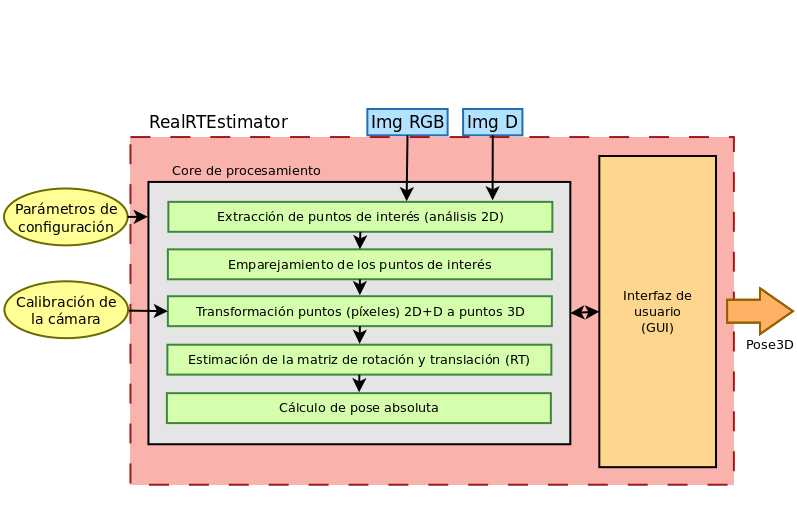
\includegraphics[scale=0.36]{Figures/diagram2.png}
\decoRule
\caption[Diagram2]{Diagrama del componente RealRTEstimator.}
\label{fig:diagram2}
\end{figure}

\begin{itemize}
\item Extración de puntos de interés (análisis 2D) del fotograma actual.

\item Emparejamientos de puntos de interés en t con respecto a los puntos extraídos en el instante anterior (t-1).

\item Transformación de puntos (píxeles) en 2D más imagen de profundidad a nube de puntos en 3D.

\item Cálculo de movimiento. Es decir, estimación de la matriz de rotación y translación (Matriz RT).

\item Calculo de pose 3D absoluta.

\end{itemize}

En las siguientes secciones desglosaremos el funcionamiento de estos diferentes bloques funcionales.

%-----------------------------------
%	SECTION Extracción de características de una imágen
%-----------------------------------
\section{Análisis 2D}

El primer bloque del componente RealRTEstimator es el de análisis 2D. A partir de dos imágenes; la imagen de color y la de profundidad, se procede a la extracción de puntos de interés.

\subsection{Detección de puntos de interés}

El término puntos de interés o detección de características (\textit{Feature Detection} en inglés) hace referencia a la tarea de localizar en una imágen puntos relevantes o carácterísticos. Estos puntos suelen ser comunes y son fáciles de seguir de fotograma en fotograma.

Para entender cuales son estos puntos característicos podemos observar un ejemplo sencillo en la Figura~\ref{fig:feature_simple}. El cuadrado azul se encuentra en una área plana, y es difícil de seguir o encontrar. En cualquier lugar por donde se desplace parecerá que es el mismo. Para el cuadrado negro, que es un borde, igual para el desplazamiento lateral, sin embargo, para el desplazamiento vertical el punto ya cambia. Por último está el cuadrado rojo, que es una esquina. Para cualquier desplazamiento de esta figura, el punto ya es diferente, lo que significa que ese punto en la figura es único y por lo tanto vamos a poder identificarlo o seguirlo en diferentes imágenes. Así pues, las esquinas suelen ser candidatos idóneos para la detección puntos de carácterísticas en una imagen (en algunos casos las manchas también pueden ser consideradas buenas zonas).

\begin{figure}[!ht]
\centering
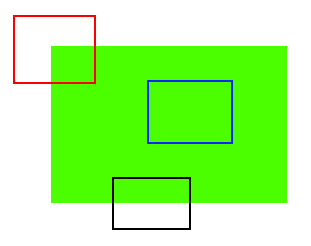
\includegraphics[scale=0.7]{Figures/feature_simple.png}
\decoRule
\caption[FeatureSimple]{Ejemplo sencillo de puntos característicos.}
\label{fig:feature_simple}
\end{figure}

Una vez entendido el concepto, el siguiente paso consiste, en averiguar cómo encontrar estos puntos de interés en una imagen real. Por ejemplo, una manera sencilla de hacerlo es buscar las regiones en las imágenes que contienen una gran variabilidad cuando son desplazadas (una pequeña distancia) hacia todas las direcciones de los alrededores.

Existen multitud de implementaciones para calcular estas carácterísticas en las imágenes. Uno de los primeros intentos en encontrar estas esquinas fue hecho por Chris Harris y Mike Stephens \parencite{Reference8}. El método, llamado \textit{Harris Corner Detector} transforma la simple idea a una fórmula matemática (\ref{eqn:Harris}) que básicamente encuentra la diferencia en intensidad por un desplazamiento (u,v) en todas las direcciones.

\begin{equation}
E(u,v)\,=\,\sum_{x,y}w(x,y)\,\,[I(x\,+\, u,\, y\,+\, v)-I(x,y)]^{2}
\label{eqn:Harris}
\end{equation}

Donde \textit{w(x,y)} es una ventana rectangular o gaussiana e I(x,y) corresponde a la intensidad. Aplicando algunos cálculos matemáticos que no vamos a entrar en detalle podemos llegar a la ecuación (\ref{eqn:Harris}) básica que determina si una ventana contiene una esquina o no.

\[ R=det(m)-k(trace(M))^{2} \]
\begin{equation}
R=\lambda_{1}\lambda_{2}-k(\lambda_{1}+\lambda_{2})^{2}
\label{eqn:Harris2}
\end{equation}

$\lambda_{1}$ y $\lambda_{2}$ son los autovalores de la matriz M, que determinarán si una región es esquina, borde o zona plana.

\begin{itemize}
\item Cuando $|R|$ es pequeño, que sucede cuando $\lambda_{1}$ y $\lambda_{2}$ son pequeños, la región es plana.

\item Cuando $R < 0$, que sucede cuando $\lambda_{1} >> \lambda_{2}$ o viceversa, la región es un borde.

\item Cuando $R$ es grande, que sucede cuando $\lambda_{1}$ y $\lambda_{2}$ son grandes y más o menos iguales, la sección es una esquina.

\end{itemize}

Más tarde, J. Shi y C. Tomasi hicieron una pequeña modificación que obtuvo mejores resultados comparados con los obtenidos en el detector de Harris \parencite{Reference9}. El resultado del detector \textit{Shi-Tomasi Corner Detector} se puede ver en la ecuación~(\ref{eqn:Shi})

\begin{equation}
R=min(\lambda_{1},\lambda_{2})
\label{eqn:Shi}
\end{equation}

Si $R$ es mayor que un determinado umbral, o dicho de otro modo; solo cuando $\lambda_{1}$ o $\lambda_{2}$ se encuentran por encima de un valor mínimo $\lambda_{min}$, se considera que cierta región es esquina. En la Figura~\ref{fig:shi_detector} se puede observar el resultado de aplicar dicho algoritmo en una imagen.

\begin{figure}[ht]
\centering
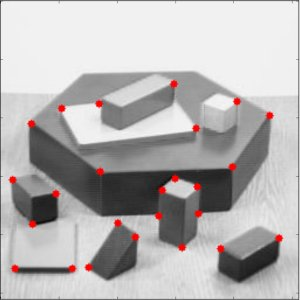
\includegraphics[scale=0.5]{Figures/shi-detector.jpg}
\decoRule
\caption[ShiDetector]{Resultado de encontrar las mejores 25 esquinas de la imagen con \textit{Shi-Tomasi Corner Detector}.}
\label{fig:shi_detector}
\end{figure}

Existen varias implementataciones para el cálculo de carácterísticas de una imagen. A parte de las mencionadas, OpenCV proporciona entre otras \textbf{SIFT} y \textbf{SURF} que son las que hemos usado para el trabajo ya que permiten además de la detección de puntos de interés, el cálculo de descriptores.

\subsection{Cálculo de descriptores}

Una vez que se conoce el punto de interés, necesitamos asignarle una huella, algo carácterístico que nos permita encontrar el mismo en otra imagen. Para ello, se procede al cálculo de descriptores (\textit{Feature Description} en inglés).

Consiste en definir la región alrededor del punto de interés para poder buscar el punto con la misma región en otra imagen. Es decir, se guarda una descripción de la región del punto dado y se busca el mismo (o el que más se parezca) a otro punto perteneciente a otra imagen.

Una vez localizado el punto se podrá llevar un seguimiento de dónde está ese punto en otra imagen. No en todos los casos, se va a encontrar un descriptor perfecto para un cierto punto, por lo que al estudiar los emparejamientos se evaluará cuanto se parecen los despriptores entre sí. Esto lo veremos con detalle en la siguiente sección.

\subsubsection{SIFT}

SIFT (Scale-Invariant Feature Transform) soluciona uno de los problemas que nos encontrabamos en los métodos anteriormente mencionados. Los métodos hasta ahora vistos para el cálculo de puntos de interés o esquinas, se suponen invariantes a la rotación, es decir, incluso si la images es rotada es posible encontrar las mismas esquinas. Esto es así porque una esquina sigue siendo una esquina si la imagen a sido rotada. Sin embargo, no contemplan los cambios de escala, un esquina no puede ser una esquina si la imagen ha sido escalada. En la Figura~\ref{fig:sift_scale_invariant} podemos ver un ejemplo de este hecho; una esquina en una pequeña imagen con una ventana no lo es cuando la imagen se amplia y se usa la misma ventana.

\begin{figure}[ht]
\centering
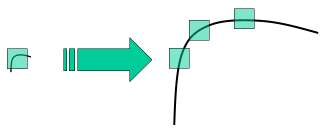
\includegraphics[scale=0.7]{Figures/sift_scale_invariant.jpg}
\decoRule
\caption[siftScaleInvariant]{Ejemplo de diferentes puntos con escala}
\label{fig:sift_scale_invariant}
\end{figure}

SIFT nace para proveer esta carencia de mano de D. Lowe \parencite{Reference10}. Un algoritmo escalarmente invariante que  localiza puntos de interés y calcula descriptores. Hay principalmente 4 etapas básicas en el algoritmo de SIFT:

\begin{enumerate}
\item \textbf{Extrema detección en espacio-escala}

Para poder detectar características en diferentes escala es necesario poder variar el tamaño de la ventana a ampliar. Para ello se utiliza un filtro de espacio-escala; un filtro LoG (Laplaciana de una Gaussiana) que con diferentes valores de $\sigma$ es capaz de detectar puntos de interés para diferentes escalas. $\sigma$ actúa como un parámetro de escala, por ejemplo como se puede ver en la FIGURA, para bajos niveles de $\sigma$ la gaussiana devuelve altos valores para las pequeñas esquinas, sin embargo, altos valores de $\sigma$ encajan bien para grandes esquinas.

Por lo tanto se busca a lo largo de la imagen y en diferentes escalas para encontrar el punto 

Así pues a lo largo de la imagen y en diferentes escalas tenemos una lista de $(x,y,\sigma)$ valores, donde $(x,y)$ representa el espacio y $\sigma$ la escala.

Sin embargo, el filtro LoG es muy costoso por lo que SIFT calcula una aproximación; la diferencia de gausianas con diferente $\sigma$ y el proceso se repetirá para diferentes octavas ($k\sigma$) como se puede apreciar en la Figura~\ref{fig:shif_dog}.

\begin{figure}[ht]
\centering
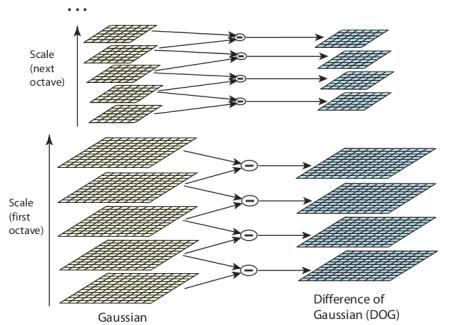
\includegraphics[scale=0.7]{Figures/sift_dog.jpg}
\decoRule
\caption[shifDog]{Proceso del cálculo de la diferencia de Gaussianas para diferentes octavas.}
\label{fig:shif_dog}
\end{figure}

Una vez obtenida la diferencia de gaussianas (DOG) se calcula el local-extrema, por ejemplo, un pixel en una imagen es comparado con sus 8 vecinos y también con los 9 píxeles en la escala anterior y la posterior 

\begin{figure}[ht]
\centering
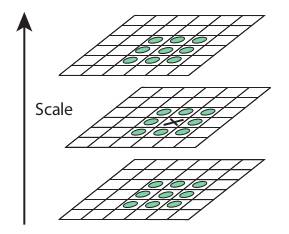
\includegraphics[scale=0.7]{Figures/sift_local_extrema.jpg}
\decoRule
\caption[siftLocalExtrema]{Proceso del cálculo de la diferencia de Gaussianas para diferentes octavas.}
\label{fig:sift_local_extrema}
\end{figure}


\item Localización de puntos de interés

bla bla balb alba 

\item Asignación de orientación

\item Descriptor del punto de interés

\item Emparejamiento de puntos

\end{enumerate}




\subsubsection{SURF}

%-----------------------------------
%	SECTION Emparejamiento (\textit{matching})
%-----------------------------------
\section{Emparejamiento (\textit{matching})}

En esta sección abordaremos las distintas estrategias que se han implementado en el componente para el emparejamiento de puntos de interés. Los emparejamientos se harán por cada imagen/fotograma que llegue de la cámara después de la extración de puntos de interés.

El componente está recibiendo continuamente imágenes del sensor, por lo que el cálculo, al igual que la extración, se hará en cada iteración. Consiguiendo así una relación entre dos fotogramas consecutivos para analizar y posteriormente cálcular el desplazamiento sucedido. Estos emparejamientos nos darán margen para desechar algunos peores emparejamientos y filtrar por los mejores utilizando diferentes técnicas. Así pues, se intentará coger los mejores emparejamientos entre una imagen en $(t)$ y otra en $(t+1)$.

Se presentarán dos soluciones para este problema; una primera solución que calcula el emparejamiento de puntos mediante un mecanismo de \textbf{Fuerza Bruta} y en segundo lugar el uso de la librería \textbf{FLANN}, ambas proporcionadas por OpenCV.

\subsection{Fuerza Bruta}

El mecanismo de Fuerza Bruta es simple. Se coge el descriptor de una de las carácterísticas del primer fotograma (imagen en $(t)$) y se comprueba el parecido con todos los puntos de carácterísticas del segundo fotograma (imagen en $(t+1)$). Estos emparejamientos se evalúan a través de un parámetro de distancia. De todas las características, el descriptor que más se parezca al primero o el emparejamiento que tenga la menor distancia es el devuelto.

Para el cálculo de este emparejamiento se usará OpenCV. En primer lugar se tendrá que crear un objeto del tipo \textit{BruteForceMatcher} y pasarle como parámetro el tipo de medida para calcular la distancia, ya que depende del tipo de descriptor a utilizar.

Una vez creado el objeto dos métodos importantes son \textit{.match()} y \textit{.knnMatch()}. El primero devuelve el mejor emparejamiento. El segundo devuelve los $k$ mejores emparejamientos, donde $k$ es definido por el usuario.

Por último, para la visualización OpenCV dispone del método \textit{.drawMatches()} que a partir de las dos imágenes y los emparejamientos obtenidos nos ayuda a dibujar los mismos para su visualización. Colocando las dos imágenes a tratar en horizontal y dibujando las líneas con los emparejamientos de una imágen a otra. En el caso de usar y querer visualizar los $k$ mejores emparejamientos existe también el método \textit{.drawMatchesKnn}.

El el siguiente ejemplo se puede observar como calcular los emparejamientos a través de OpenCV

\begin{lstlisting}[style=CStyle]
// matching descriptors
BruteForceMatcher<L2<float> > matcher;
vector<DMatch> matches;
matcher.match(descriptors1, descriptors2, matches);
\end{lstlisting}


\subsection{FLANN}

%-----------------------------------
%	SUBSECTION Cálculo de movimiento
%-----------------------------------
\section{Cálculo de movimiento}

\subsection{Matriz RT}

%-----------------------------------
%	SECTION Interfaz gráfica
%-----------------------------------
\section{Interfaz gráfica}